
\documentclass[a4paper,11pt]{report}

\usepackage{amsmath}
\usepackage{amssymb}
\usepackage[utf8x]{inputenc}
\usepackage{fullpage}
\usepackage[hyphens]{url}
%\usepackage{hyperref} %this messes up the line breaks of url
\usepackage{xspace}
\usepackage{graphicx}
\usepackage{longtable}
\usepackage{subfigure}
\usepackage{listings}

%%commands
\newcommand{\sname}{QRSim\xspace}
\newcommand{\snamettt}{\texttt{QRSim}\xspace}

\newcommand{\webrepo}{\url{http://complacs.cs.ucl.ac.uk/complacs/simulator/qrsim-lastStable.zip}\xspace}
\newcommand{\webman}{\url{http://complacs.cs.ucl.ac.uk/complacs/simulator/manual.pdf}\xspace}

\newcommand\mytexttt[1]{\texttt{\hyphenchar\font=45\relax #1}}
\newcommand{\nn}{\nonumber}
\newcommand{\pr}{{\rm Pr}}


% Title Page
\title{{CompLACS} Helicopters Scenarios}
\author{Renzo De Nardi,\\University College London\\\texttt{rdenardi@cs.ucl.ac.uk}}

\begin{document}
\maketitle



\begin{abstract}
This document describes the three types of scenarios devised at UCL to develop and test learning and control algorithm with application to a flock of autonomous quadrotor helicopters, one of the three real world platforms of the {CompLACS} project.
The three application scenarios are explicitly chosen to expose different types of challenges that occur in the domain of multi-platform aerial robotics so to provide a variety of opportunities for investigation.

This report is divided into three parts one for each of the three scenarios; each part gives a formal description of the scenario in terms of its setup, its objective, and its variations. 

In order to aid the development and testing of learning algorithms, we provide a simulation environment based on the \sname quadrotor simulator for each the scenarios along with handy code examples.

Since the scenarios simulations are built on top of \sname, we refer to its manual (\webman) for details about the simulator and its API.

\end{abstract}

\tableofcontents

\chapter{Quadrotors Scenarios}

\section{Scenario 1: Cats and Mouse Game}

The first of the scenarios is designed to focus primarily on the challenges encountered in the coordinated control of multiple UAVs; the associated problems of sensing and state estimation are somewhat simplified by the choice of task, environment and platform sensors. 

\subsection{Description}
The task to be accomplished in this scenario is in the form of a team game in which $N$ helicopters (cats) have to surround and effectively trap (i.e. get close to) another helicopter (mouse) at the end of the allotted time. 

For simplicity the task is assumed to take place in an area devoided of obstacles so that helicopters can fly freely. Getting in contact with the ground or another UAV will however produce a collision.
The platforms are equipped with noisy sensors so only observation of the vehicle state are available.  
Depending on the circumstances wind and other aerodynamic disturbances that affect the flight behaviour might be present in the flying area.

Snapshots of the initial ($t=0$) and terminal ($t=T$) configurations from a typical successful run are visible in figures \ref{fig:catmousestart} and \ref{fig:catmousestop} respectively. 

In the next section we give a more formal description of the problem.

\begin{figure}[ht]
\centering
\subfigure[$t=0$]{
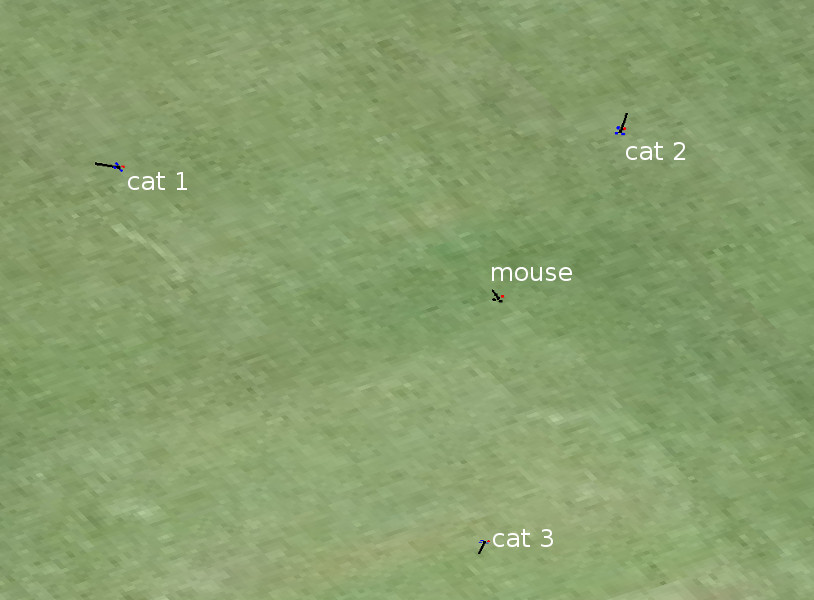
\includegraphics[width=0.48\textwidth]{fig/catmousestart.jpg} 
\label{fig:catmousestart}}
\subfigure[$t=T$]{
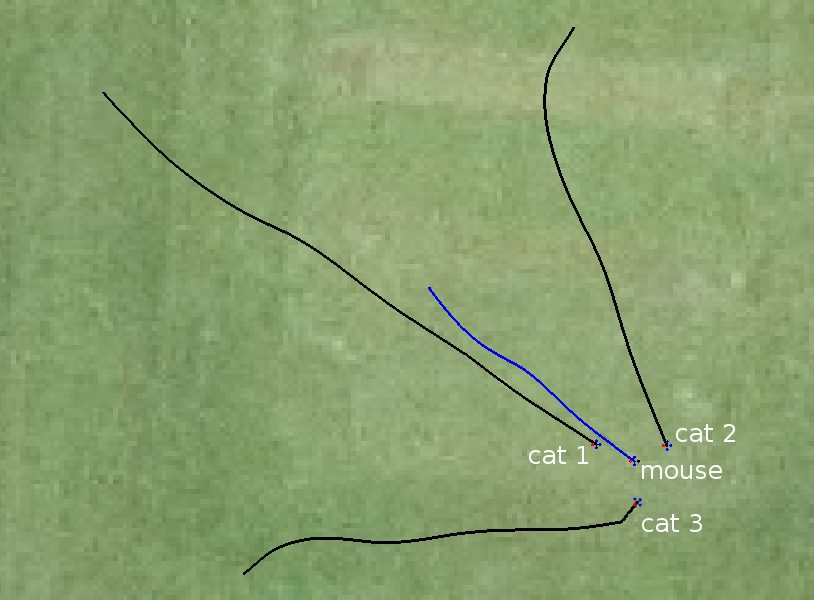
\includegraphics[width=0.48\textwidth]{fig/catmousestop.jpg}
\label{fig:catmousestop}}
\caption{Typical successful run: start(a) and end(b) configurations. \label{fig:catmouse}}
\end{figure}

\subsection{MDP}

The system underlying the task is modelled as a discrete time, finite horizon MDP on a continuous state space. The system runs from $t=0$ to $t=T$ with a time step equivalent to $1s$ of simulated time\footnote{The update rate is user-configurable with default value of 1Hz.}. 

\paragraph{State:} The state $s_t = (x^1_t,...,x^{N}_t,x^m_t)$ at time $t$ comprises of the state vectors of all the cats ($x^1,...,x^{N}$) and of the mouse ($x^m$) helicopters. 
Each platform state contains in turn the position ($[p_x,p_y,p_z]^\intercal$), velocity ($[u,v,w]^\intercal$), orientation ($[\phi,\theta,\psi]^\intercal$) and rotational velocity ($[p,q,r]^\intercal$) of the platform:
\begin{align}
x = [p_x,p_y,p_z,\phi,\theta,\psi,u,v,w,p,q,r]\intercal .
\end{align}
 All of these are continuous variables (see section \ref{CatMouseSim} for more details).

The environment is itself three dimensional although we will see (section \ref{catmouseactions}) that the helicopters are assumed to fly at a fixed altitude.

\paragraph{Initial State:} At the beginning of the task the mouse is placed at the origin of the flight space\footnote{Without loss of generality since the control problem depends on the relative positions of mouse and cats as long as the flying area is sufficiently large.} and the cats are positioned randomly around the mouse.

The initial positions of cats are generated as:
$$
\left[
\begin{array}{l}
p^i_x \\
p^i_y \\
p^i_z \\
\end{array}
\right]_0
= \left[
 \begin{array}{l}
 p^m_x \\
 p^m_y \\
 0 
 \end{array}
 \right] + 
 \left[
 \begin{array}{l}
d_i \cos(\alpha_i) \\
d_i \sin(\alpha_i) \\
- h_{fix} \\
\end{array}
\right] \qquad i \in 1..N
$$
where $\alpha_i \sim \mathcal{U}(0,2\pi)$, $d_i \sim \mathcal{U}(D_m,D_M)$ and $\mathcal{U}(a,b)$ indicates a uniform distribution over the interval $[a,b]$. The minimum and maximum distance from the mouse $D_m,D_M$ and the altitude $h_{fix}$ are user-configurable.
An additional parameter $D_{c2c}$ allows to define a minimum distance between any two cats; this prevent the occurrence of an initial state in which two cats are too close.

At $t=0$ all the helicopters are stationary (i.e. their velocities are zero).

\paragraph{Actions:}\label{catmouseactions} 
A real quadrotor of the type considered in our task generally presents four continuous control inputs (i.e. pitch, roll, yaw angles and throttle) which needs to be updated at a rate of $50Hz$. Even with a moderately long time horizon the control space becomes rather large.

To limit the space of control inputs, in our setup each UAV is equipped with a close loop PID controller that accepts 2D linear velocity commands $a^i_t=[v^i_x,v^i_y]^\intercal$ (in global coordinates) and combines them with the estimated platform velocity to produce the necessary attitude and throttle commands for the platform. The PID accepts commanded velocity at a rate of $1Hz$ and provides the platform controls at $50Hz$.
To additionally reduce the control space the PID takes also care of maintaining a constant altitude and heading\footnote{The use of a PID controller in addition to reducing the number of control inputs makes the task closer to what is possible to implement and test using real quadrotors.}. 

The reduced action space $a_t$ at time $t$ comprises of the 2D linear velocity commands for each of the cats helicopters:
\begin{align}
a_t = (a^1_t,...,a^{N}_t).
\end{align}

\paragraph{Dynamics:} 
The task has a Markovian transition dynamics defined by $P(s_{t+1}|s_t,a_t)$ which denotes the conditional density of state $s$ at time $t+1$ given state-action $(s_t,a_t)=(s,a)$ at time~$t$.

In the case of the cats helicopters the transition dynamics is defined by the combination of PID velocity controllers, platforms dynamics, sensor and wind dynamics (since these in turn effect the quadrotor) all of which are part of the \sname simulator\footnote{We refer to the \sname manual for details.}. 

For the mouse helicopter the transition dynamics is 
not only based on the platform dynamics but also by the way the mouse moves in response to the cats.

 As the task starts the mouse helicopter tries to escape the cats by moving at a constant (max) speed\footnote{While the control law that governs the quadrotor attempts to maintain a fix maximum speed, in practice the true speed will not be constant due to sensor noise wind disturbance and dynamic effects.} and choosing a direction that prioritize escaping from the closer cats.
In specific the 2D velocity action for the mouse at time $t$ is computed as:
\begin{equation}\label{eqn:mousectrl}
\begin{array}{ll}
a^m_t = V_{M} \frac{\mathsf{v}_t}{\| \mathsf{v}_t \|} &
\text{where } \;\;\mathsf{v}_t = \sum_{i=1}^N \frac{\left[\begin{array}{c} p^i_x \\ p^i_y \end{array}\right]_t - \left[\begin{array}{c} p^m_x \\ p^m_y \end{array}\right]_t}{\left\| \left[\begin{array}{c} p^i_x \\ p^i_y \end{array}\right]_t - \left[\begin{array}{c} p^m_x \\ p^m_y \end{array}\right]_t \right\|^2}
\end{array}
\end{equation}
and $V_{M}$ is the (user-configurable) maximum speed that the mouse can achieve. 

Different control strategies could be considered for the mouse; in practice the one considered in equation \ref{eqn:mousectrl} is both simple and has shown to be sufficient to provide for a challenging task.

\paragraph{Observations}
The helicopter state $x^i_t$ is observed directly although depending on the specific task variation (see Section~\ref{CatMouseVariations}) the state variables might be affected by stochastic noise.
For more details about the noise models used by \sname we refer the reader to the simulator manual. 

\paragraph{Reward:}
The cats are successful if they are able to trap the mouse at the end of the task; a meaningful final reward can be defined as the sum of the squared (2D) distances\footnote{$d_{2D}(x^i_T,x^m_T) = \Vert[p^i_x,p^i_y]_T^\intercal - [p^m_x,p^m_y]_T^\intercal\Vert$.} between the cats and the mouse at time $T$:
$$r_T = - \sum^N_{i=1} d_{2D}(x^i_T,x^m_T)^2.$$
A large negative reward\footnote{The default value of the negative reward is $-1000$ but it can be configured by the user.} is returned if any of the helicopters (including the mouse) goes outside of the flying area or if any collision happens during the task.

\subsection{Task Variations} \label{CatMouseVariations}
The difficulty of the considered control problem depends on the level of sensor noise and wind disturbance; so we define three versions of the task with increasing level of realism (and consequently difficulty):
\begin{itemize}
 \item \textit{\textbf{1A} noiseless:} the dynamics of the quadrotors is deterministic and the state returned is the true platform state;
 \item \textit{\textbf{1B} noisy:} the dynamics of the quadrotors is stochastic and the state returned is a noisy estimate of the platform state (i.e. with additional correlated noise);
 \item \textit{\textbf{1C} noisy and windy:} the dynamics of the quadrotors is stochastic and affected by wind disturbances (following a wind model), the state returned is a noisy estimate of the platform state (i.e. with additional correlated noise).
\end{itemize}

\subsection{Simulation Code}\label{CatMouseSim}
The cat and mouse scenario can be promptly defined on top of the \sname simulator by means of dedicated task classes\footnote{Refer to the \sname manual for details on task classes.}. In specific we make available one task class for each of the three scenario variations introduced in section \ref{CatMouseVariations}:
\begin{itemize}
\item\textit{1A}: \mytexttt{TaskCatsMouseNoiseless.m},
\item\textit{1B}: \mytexttt{TaskCatsMouseNoisy.m},
\item\textit{1C}: \mytexttt{TaskCatsMouseNoisyAndWindy.m}. 
\end{itemize}

Commenting the code in details is beyond the scope of this report but it is useful to briefly outline which task methods are responsible for handling the various task specific components:
\begin{itemize}
\item\mytexttt{init()}: defines all the platforms and sensor parameters;
\item\mytexttt{reset()}: defines the UAVs starting condition;
\item\mytexttt{step(U)}: defines the mouse evasion strategy and uses the PID controllers to transform velocity commands into angle command to the helicopters;
\item\mytexttt{reward()}: defines the task reward.
\end{itemize}

Listing \ref{lst:mcm} (file \texttt{main\_catsmouse.m}) shows the set of steps that are necessary to run a scenario task.
\begin{lstlisting}[float=ht!bp,caption=main\_catsmouse.m,language=Matlab,frame=lines,label=lst:mcm,numbers=left,basicstyle=\small]
qrsim = QRSim();

% load task parameters and do housekeeping
state = qrsim.init('TaskCatsMouseNoisyAndWindy');

U = zeros(2,state.task.Nc);

% run the scenario and at every time step generate a control
% input for each of the uavs
for i=1:state.task.durationInSteps,
    
    % get the mouse position (note id state.task.Nc+1)
    mousePos = state.platforms{state.task.Nc+1}.getEX(1:2);
    
    % quick and easy way of computing velocity controls for each cat 
    for j=1:state.task.Nc,
	collisionDistance = state.platforms{j}.getCollisionDistance();
		
        % vector to the mouse
        u = mousePos - state.platforms{j}.getEX(1:2);
        
        % add a weighted velocity (i.e. "predict" where the mouse will be)
        u = u  + (norm(u)/2)*state.platforms{state.task.Nc+1}.getEX(18:19);
        
        % keep away from other cats if closer than 2*collisionDistance        
        for k = 1:state.task.Nc,
            if(state.platforms{k}.isValid())                  
                d = state.platforms{j}.getEX(1:2) 
                    - state.platforms{k}.getEX(1:2);
                if((k~=j)&&(norm(d)<2*collisionDistance))
                    u = u + (1/(norm(d)-collisionDistance()))*(d/norm(d));
                end
            end
        end
        
        % scale by the max allowed velocity
        U(:,j) = state.task.velPIDs{j}.maxv*(u/norm(u));
    end
    
    % step simulator
    qrsim.step(U);
end

% get final reward
fprintf('final reward: %f\n',qrsim.reward());

\end{lstlisting}

After the desired task is initialized (line 4), a basic for loop is executed for the number of time steps specified by the task. Within the loop the 2D velocity control is computed for each helicopter and passed to the corresponding PID (line 37). 
In our listing we show a simple (and suboptimal) scheme in which the velocity direction of each cat directly towards the future mouse position mouse (line 20-23) but that also keeps away from neighbouring cats (line 26-34). 
The helicopter control inputs produced by the PID controllers are then used to step the simulator (line 41).
Finally after the execution of the task is concluded, the final reward for the task can be retrieved (line 46).

We remind the reader that within the simulator the helicopter state $x^i_t$ is denoted as \texttt{eX}:
$$\texttt{eX} = [\tilde{p}_x,\tilde{p}_y,\tilde{p}_z,\tilde{\phi},\tilde{\theta},\tilde{\psi},0,0,0,\tilde{p},\tilde{q},\tilde{r},0,\tilde{a}_x,\tilde{a}_y,\tilde{a}_z,h,\dot{p}_x,\dot{p}_y,\dot{h}]^\intercal$$
while the actions $a^i_t$ are denoted as controls \texttt{u}:
$$\texttt{u}=[v_x,v_y]^\intercal$$
with the variables defined in section \ref{tab:naming}.

The task, the configurations and the example main files are in the directory \mytexttt{scenarios/catsmouse} within the \sname simulator. 

\newpage
\section{Scenario 2: Search and Rescue}
The second scenario is designed explicitly to expose the complex interplay between sensing and acting typical in autonomous robotics task. To solve the task the agent/s has to perform inference about the state of the environment given some observations and take actions based on its belief. 

\subsection{Description}
The task to be accomplished in this scenario is in the form of a wilderness search and rescue mission; several targets (people) are lost/injured on the ground in a landscape and need to be located and rescued. 

In addition to its navigation sensors each helicopter agent taking part in the search 
is equipped with a camera/classification module that allows it to detect the presence of targets in its field of view. Rather than raw images the camera module provides higher-level data in the form of log likelihood ratios for the current observation conditioned on the presence or absence of a target. The quality of detection depends upon the ground type and the geometry between helicopter and ground (e.g. the distance).  

The search area is limited but its extent is so that a trivial lawn mower pattern of search will not allow covering all the area in the allotted time. The landscape has different types of terrain; persons are more likely to be present on some class of terrain than others. The persons are assumed to not move during the task. 

Additionally we assume that the flying area is free of obstacles so that the UAVs can move freely in the 3D space. Getting in contact with the ground or another UAV will however produce a collision.

A snapshot from a typical run is shown in figure \ref{fig:searchrescue} along with an example of the observation returned by the camera/classifier model.
\begin{figure}[ht]
\centering
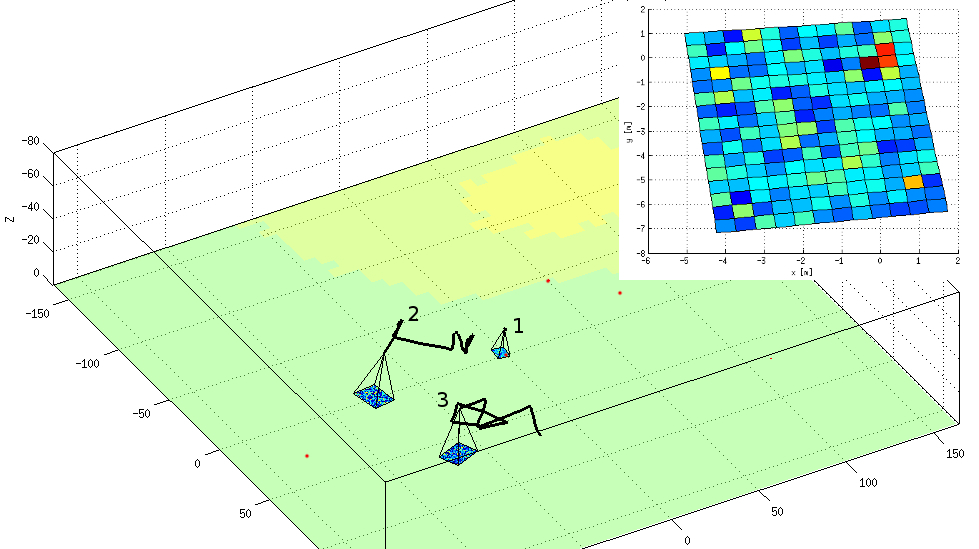
\includegraphics[width=15cm]{fig/searchrescue.jpg}
\caption{Search and rescue run with three helicopters; note the different terrain types (denoted by different colors) and the persons (red dots). The insert shows the camera observation from UAV 1 that happens to be over a person. \label{fig:searchrescue}}
\end{figure}

\subsection{MDP}
The system underlying the task is modelled as a discrete time, finite horizon MDP on a continuous state space. The system runs from $t=0$ to $t=T$ with a time step equivalent to $1s$ of simulated time\footnote{The update rate is user-configurable with default value of 1Hz.}.

\paragraph{States:} The state $s_t=(x^1_t,...,x^{N}_t,b^1_t,...,b^P_t)$ at time $t$ comprises the helicopters state vectors $x^i_t$ and the location of the $P$ targets $b^j_t$.

Each platform state contains in turn the position ($[p_x,p_y,p_z]^\intercal$), velocity ($[u,v,w]^\intercal$), orientation ($[\phi,\theta,\psi]^\intercal$) and rotational velocity ($[p,q,r]^\intercal$) of the platform:
\begin{align}
x = [p_x,p_y,p_z,\phi,\theta,\psi,u,v,w,p,q,r]\intercal .
\end{align} 
The environment is itself three dimensional and the helicopter can freely move in three dimensions.

The person's location is expressed in terms of its coordinate w.r.t. the global reference frame  $b^j=[p^j_x,p^j_y,0]^\intercal$; the person's $z$ coordinate is zero since we assume that the ground is flat and that the targets are located on the ground.

\paragraph{Initial State:} At the beginning of the task a new terrain map is generated based on the number of terrain classes and split between class types specified by the user\footnote{The user specifies what percentage of the total area belongs to each class.}. 
The extent of the flying area is scaled accordingly to the number of platforms and time horizon in order to ensure that the task is nontrivial.

Subsequently a number of persons is randomly placed in the search area. The user can control where persons are placed by specifying the probability of a target to be located on a specific terrain class\footnote{Each person's location is generated independently.}. 

Finally the helicopters are located randomly (with uniform probability) around the flying area at the nominal flight height\footnote{The initial altitude can be configured by the user but is set to a $25m$ default value.}.

\paragraph{Actions:}
At each time step the agent specifies an action $a^i_t$ for each of the UAVs taking part in the task; the action is expressed in terms of a 3D velocity vector in global NED coordinates:
\begin{align}
a^i_t=[v^i_x,v^i_y,v^i_z]_t^\intercal \qquad\qquad i\in[1..N].
\end{align}

Similarly to what explained for in section \ref{catmouseactions} the actions are nothing more than set points to a PID controller that attempts to fly the UAV at the requested velocity.
Due to delays and disturbances mismatches between the commanded and the actual velocity of the UAV have to be expected. 

\paragraph{Dynamics:}\label{rescued} For the UAVs the transition dynamics is defined by the combination of PID velocity controllers, platforms dynamics, sensor and wind dynamics (since these in turn effect the quadrotor) all of which are specified by the \sname simulator. Such transition dynamics are Markovian and defined by $P(x_{t+1}|x_t,a_t)$ which denotes the conditional density of state $x$ at $t+1$ given $(x_t,a_t) = (x,a)$ at time $t$.
The dynamics of the UAVs is independent of the targets $b^j_t$.

Targets $b^j$ are stationary unless a helicopter hovers (i.e. its speed is low) sufficiently close to it, in which case the target is considered rescued and removed from the environment.
More formally:
\begin{align}
\begin{array}{l l}
if ~ \exists ~ i,j~:~ d_{3D}\left( x^i_t,b^j_t \right) < \delta ~ \wedge ~\and \parallel [u^i,v^i,w^i]_t^\intercal \parallel < \epsilon & \\
 \Rightarrow \quad P=P-1 & i\in\{1,...,N\},j\in\{1,...,P\} 
\end{array}
\end{align}
where $d_{3D}$ is the standard Euclidean distance in three dimensions\footnote{Defined as $$d_{3D}(x_t,b^j_t) = \parallel b^j_t -[p_x,p_y,p_z]_t^\intercal \parallel.$$} and $(\epsilon,\delta)$ are user specified thresholds\footnote{The default values for the distance threshold and the speed threshold are $\delta=5m$ and $\epsilon=0.1m/s$}.

\paragraph{Observations}

The helicopter state $x_t$ is observed directly although depending on the specific task variation (see Section~\ref{SearchRescueVariations}) the state variables might be affected by stochastic noise.

The position of the targets $b^j_t$ is not known, but observations $o_t$ are provided by the camera at each time step.

Following standard object detection techniques we assume that the incoming image (at time $t$) is split into $M_t$ windows $\{w^k_t\}^{M_t}_{k=1}$  (of size informed by the current altitude and an assumed fixed size for the person) which are then analysed for targets. 
Given the current UAV pose $x_t$ and the fixed camera parameters the set of windows projects on the ground to a set of $M$ patches $\{g^k_t\}^{M_t}_{k=1}$. 
More precisely this assumes that a map is available and that the mapping
\begin{align}
\{g^k_t\}^{M_t}_{k=1} \mapsto \{w^k_t\}^{M_t}_{k=1}\nn
\end{align}
is known, but does not have to be considered explicitly by the agent. 

We assume that some form of person detection algorithm is run on each of the image windows ${w^k_t}$. As a result it is possible to evaluate the probability that such image patch was originated by a person (at the corresponding ground location $g^k_t$) versus the probability that ${w^k_t}$ was originated by clear ground at location $g^k_t$; what is commonly called a likelihood ratio.

To generate likelihood ratios we use a model learned from the scores obtained by running an off the shelf person classifier on aerial images dataset collected with the quadrotor UAV in use at UCL. We refer to section \ref{personclassifier} for more details about such model.

The observation $o_t$ is simply the collection of the log likelihood ratios obtained for each of the image windows ${w^k_t}$ (and therefore also for the corresponding ground patches $g^k_t$):
\begin{align}
o_t = \left\{\log
\left(
\frac{\pr(\mbox{image at time } t~|~\mbox{target in } g^k_t \mbox{, UAV at }x_t)}
{\pr(\mbox{image at time }t~|~\mbox{no target in } g^k_t \mbox{, UAV at }x_t)}
\right)
\right\}^{M_t}_{k=1}. \nn
\end{align}

An example of the observation returned by our simulated scenario is visible in the insert of figure \ref{fig:searchrescue}. A higher value of the ratio (red colour) is noticeable for the ground patches that are at the person location; also note how the patches are conveniently expressed in ground coordinates.

\paragraph{Reward:} 
The reward $r_t$ for the task is designed to prize the UAVs for quickly rescuing targets. In this spirit $r_t$ at time $t$ is defined to be $1$ when a helicopter hovers sufficiently close to a target and a small negative value otherwise.
More formally:
\begin{align}
r_t =  \left\{
\begin{array}{c l}
1 & if ~ \exists ~ i,j~:~ d_{3D}\left( x^i_t,b^j_t \right) < \delta ~ \wedge ~\and \parallel [u,v,w]_t^\intercal \parallel < \epsilon \quad i\in\{1,...,N\},j\in\{1,...,P\}\\
-1/T & otherwise
\end{array}
\right.
\end{align}
where $T$ is the task duration $T$ and $\epsilon,\delta$ are respectively the distance and velocity thresholds that define a person as rescued (see section \ref{rescued}). 
A large negative reward\footnote{The default value of the negative reward is $-1000$ but it can be configured by the user.} is returned if the helicopter goes outside of the flying area or if any collision happens during the task. 

\subsection{Task Variations} \label{SearchRescueVariations}
The difficulty of solving the task depends on the number of platforms that are employed as well as on the level of sensor noise and wind disturbance; we provide four versions of the task with increasing level of difficulty:
\begin{itemize}
 \item \textit{\textbf{2A} single helicopter noiseless:} only one helicopter is used for the search, its dynamic is deterministic and the state returned is the true platform state;
 \item \textit{\textbf{2B} single helicopter noisy:} only one helicopter is used for the search, its dynamics is stochastic and the state returned is a noisy estimate of the platform state (i.e. with additional correlated noise);
 \item \textit{\textbf{2C} multiple helicopters noiseless:} several helicopters are used for the search, their dynamics is deterministic and the state returned is the true platform state;
 \item \textit{\textbf{2D} multiple helicopters noisy and windy:} several helicopters are used for the search, their dynamics is stochastic and affected by wind disturbances (following a wind model), the state returned is a noisy estimate of the platform state (i.e. with additional correlated noise).
\end{itemize}

\subsection{Simulation Code} \label{SearchRescueSim}

A simulated version of each of the variations of this scenario is made available in the form of a task class that can be readily used within the \sname helicopter simulator. 
More specifically the four task variations presented in section \ref{SearchRescueVariations} are named:
\begin{itemize}
\item\textit{2A}: \mytexttt{TaskSearchRescueSingleNoiseless.m}, 
\item\textit{2B}: \mytexttt{TaskSearchRescueSingleNoisy.m}, 
\item\textit{2C}: \mytexttt{TaskSearchRescueMultipleNoiseless.m} 
\item\textit{2D}: \mytexttt{TaskSearchRescueMultipleNoisyAndWindy.m}. 
\end{itemize}

Commenting the code in details is beyond the scope of this report but it is useful to briefly outline which task methods are responsible for handling the various task specific components:
\begin{itemize}
\item\mytexttt{init()}: defines all the platforms, sensor and environment parameters;
\item\mytexttt{reset()}: defines the task starting condition for UAVs and persons;
\item\mytexttt{step(U)}: uses the PID controllers to transform velocity commands into angle command to the helicopters, checks if a target was located and removes it;
\item\mytexttt{reward()}: returns the reward at the current time step;
\item\mytexttt{getNumberOfPersons()}: returns the number of persons present at the beginning of the task.
\end{itemize}

We also provide the example file \texttt{main\_searchrescue.m} (listing \ref{lst:msr}) which briefly shows how to initialize and run any of the search and rescue tasks.
\begin{lstlisting}[float=ht!bp,caption=main\_searchrescue.m,language=Matlab,frame=lines,label=lst:msr,numbers=left,basicstyle=\small]
% create simulator object
qrsim = QRSim();

% load task parameters and do housekeeping
state = qrsim.init('TaskSearchRescueSingleNoiseless');

% create a 3 x helicopters matrix of control inputs
% column i will contain the 3D NED velocity [vx;vy;vz] for helicopter i
U = zeros(3,state.task.numUAVs);

% number of persons to locate in this task        
np = state.task.getNumberOfPersons();

% run the scenario and at every time step generate a control
% input for each of the uavs
for i=1:state.task.durationInSteps,    
    % random search policy in which the helicopter(s) moves around
    % at a fixed velocity changing direction every once in a while    
    if(rem(i-1,10)==0)
        for j=1:state.task.numUAVs,     
            if(state.platforms{j}.isValid()) 
                % random velocity direction
                u(:,j) = rand(2,1)-[0.5;0.5];
                % fixed velocity 0.5 times max allowed velocity
                U(:,j) = [0.5*state.task.velPIDs{j}.maxv*...
                          (u(:,j)/norm(u(:,j)));0];
                
                % if the uav is going astray we point it back to the center
                p = state.platforms{j}.getEX(1:2);
                if(norm(p)>100)
                    U(:,j) = [-0.8*state.task.velPIDs{j}.maxv*p/norm(p);0];
                end
            end
        end
    end
    
    % step simulator
    qrsim.step(U);
    
    % get camera measurements:
    % the output is an object of type CemeraObservation, i.e.
    % a simple structure containing the fields:
    % llkd      log-likelihood difference for each ground patch
    % wg        list of corner points for the ground patches
    % gridDims  dimensions of the grid of measurements    %
    for j=1:state.task.numUAVs,
        m = state.platforms{j}.getCameraOutput();
    end   
    
    % reward (1 as soon as we hovering close enough to a person)
    r = qrsim.reward();
end
\end{lstlisting}
The layout of the code is very similar to what we have seen for the cats and mouse scenarios; after a preliminary initialization (lines $2-9$), a for loop takes care of stepping the simulation (line $38$) for the predefined number of time steps.
For simplicity in this example, the UAVs move in the space at a fix velocity changing their direction randomly every $10$ time steps (lines $19-35$).
For each UAV the camera measurement can be retrieved after stepping the simulator with a new action (line $47$). In a more interesting policy than the random one we are showing in this example an agent would make use of this new observation (and of the previous) to decide its next action.
Lastly line $51$ shows how to retrieve the reward at the current time step. 

In some situations it might be useful to know the total number of targets present in the environment, line $12$ shows how is possible to do that using the \texttt{getNumberOfPersons()} method.
 
We remind the reader that within the simulator the helicopter state $x^i_t$ is denoted as \texttt{eX}:
$$\texttt{eX} = [\tilde{p}_x,\tilde{p}_y,\tilde{p}_z,\tilde{\phi},\tilde{\theta},\tilde{\psi},0,0,0,\tilde{p},\tilde{q},\tilde{r},0,\tilde{a}_x,\tilde{a}_y,\tilde{a}_z,h,\dot{p}_x,\dot{p}_y,\dot{h}]^\intercal$$
while the actions $a^i_t$ are denoted as controls \texttt{u}:
$$\texttt{u}=[v_x,v_y,v_z]^\intercal$$
with the variables defined in section \ref{tab:naming}.

The task, the configurations and the example main files are in the directory \mytexttt{scenarios/searchrescue} within the \sname simulator.

\newpage
\section{Scenario 3: Plume Modelling}\label{plumemodelling}
In the third and last scenario we design tasks in which sensing and estimation of the target environment play a crucial role. In specific the actions of the agent are aimed at generating reliable predictions about the flying area.  

\subsection{Description}

In this scenario we envisage the situation in which a plume is dispersed in the flying area and we are interested in using one or more UAVs to estimate the plume concentration\footnote{Hereby we simply refer to concentration, in a real environment this would be a property of the plume that can be realistically measured e.g. CO concentration.}.

Depending on the task settings (see section \ref{PlumeVariations}) one or more sources might be present in the environment and the plume distribution might evolve over time. Any wind affects both the UAV flight behaviour and the plume distribution.
UAVs are equipped with noisy navigation sensors that allow observing their location, attitude and velocities and also with a sensor that produces noisy observation of the plume concentration. 

The plume concentration follows a known model but with unknown parameter values; the task objective is to provide a concentration estimate $\hat{c}_T$ at some pre-specified time $T$. 
For this scenario we selected three main classes of concentration models; they were chosen for being widely adopted (\cite{stockie2011}) while remaining relatively simple:
\begin{itemize}
\item \textit{Gaussian}: when no wind is present in the flying area and the source emits plume with a constant rate, the plume disperses around the source and its concentration can be described by a three dimensional Gaussian (equation \ref{eqn:singlesourcegaussian}). Since the source emits at constant rate the resulting dispersion pattern is static, however to make the model not completely trivial we assume that the dispersion is not necessarily isotropic; Figure\ref{fig:singlegaussplume} depicts an example of type of concentration pattern produced by this model.
\item \textit{Gaussian Dispersion}: when wind is present in the flying area, and the source emits plume with a constant rate, the plume is blown downwind and disperses as it gets farther from the source. The concentration takes a cone like shape which expands as the distance from the source increases (equation \ref{eqn:singlesourcegaussiandispersion}). In the case in which the mean wind velocity and direction do not change with time\footnote{This will be the case in our settings.}, the resulting concentration is also time invariant. An example of the resulting dispersion is visible in Figure\ref{fig:multigaussplume}.
\item \textit{Gaussian Puff Dispersion} when wind is present in the flying area but the source emits plume for short time intervals (i.e. short puffs), each puff travels downwind expanding as it gets farther from the source. At every time instant the resulting concentration is the superposition of the many puffs (equation \ref{eqn:singlesourcesgaussianpuffdispersion}); the concentration is therefore time variant.  Figure \ref{fig:singlegausspuffplume} shows an example of such dispersion model.
\end{itemize}
For each type of dispersion model the case in which more than one source is present in the environment can be considered simply by superimposing the effects of several individual sources; superposition gives origin to substantially more complex distributions.

As in the previous tasks we assume that the flying area is free of obstacles so that the UAVs can move freely in the 3D space. Getting in contact with the ground or another UAV will however produce a collision.

\textit{Note:}
Since the dispersion models are known, one possible way to solve the tasks is to estimate the model parameters (or a distribution over them). While this is an appropriate solution we emphasize that the agent is not required to solve the task in this way and so model agnostic way of producing concentration estimations are equally appropriate. 

\begin{figure}[t]
\centering
\subfigure[Single source Gaussian concentration.]{
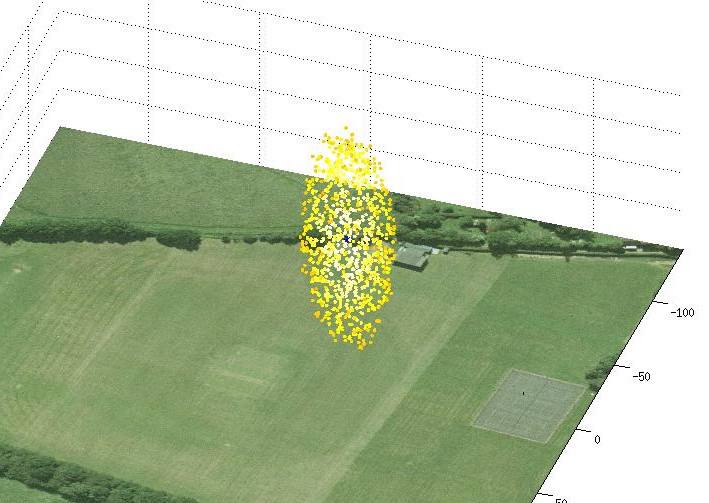
\includegraphics[width=0.48\textwidth]{fig/singlegaussplume.jpg}
\label{fig:singlegaussplume}}
\subfigure[Multiple sources Gaussian dispersion.]{
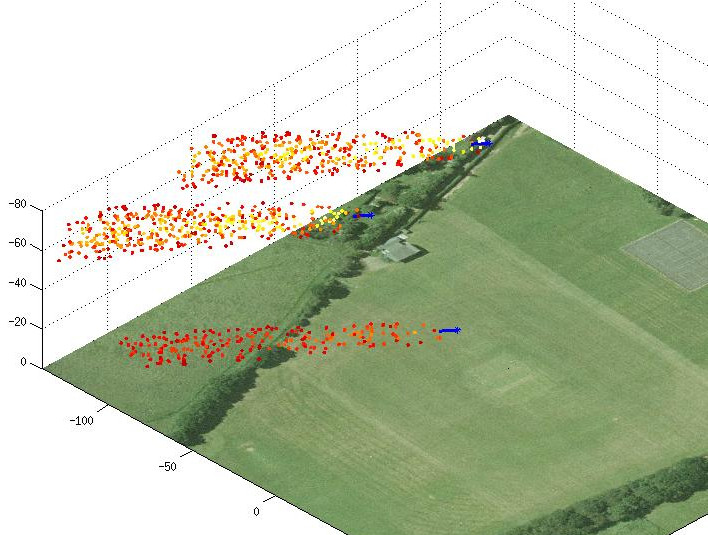
\includegraphics[width=0.48\textwidth]{fig/multigaussplume.jpg}
\label{fig:multigaussplume}}
\subfigure[Single source Gaussian puff dispersion.]{
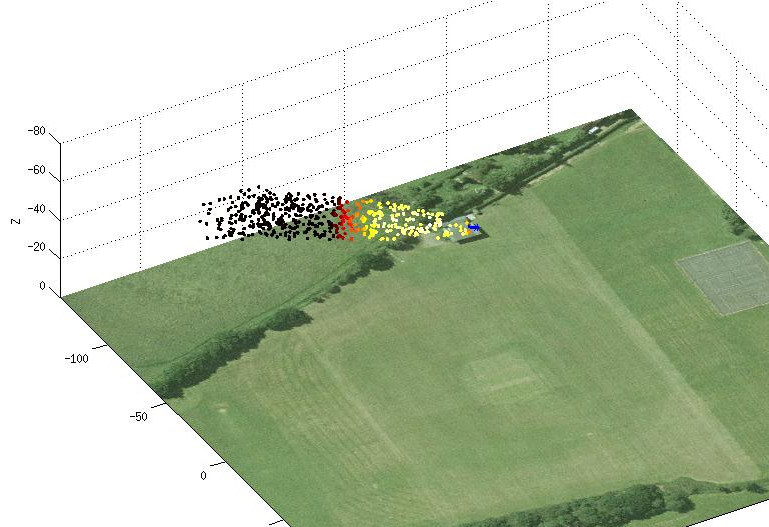
\includegraphics[width=0.48\textwidth]{fig/singlegausspuffplume.jpg}
\label{fig:singlegausspuffplume}}
\caption{Plume models; darker markers indicate lower concentration.\label{fig:plume}}
\end{figure}

\subsection{MDP}
The system underlying the task is modelled as a discrete time Markov process on a continuous state space. The system is updated at a frequency of 1Hz\footnote{The update rate is user-configurable with default value of 1Hz.} and the task has a duration $T$.

\paragraph{States:} the state $s_t=(x^1_t,..,x^N_t,c_t)$ at time $t$ comprises the helicopter/s state $x^i_t$ and the plume concentration $c_t$.
Each platform state contains in turn the position ($[p_x,p_y,p_z]^\intercal$), velocity ($[u,v,w]^\intercal$), orientation ($[\phi,\theta,\psi]^\intercal$) and rotational velocity ($[p,q,r]^\intercal$) of the platform:
\begin{align}
x = [p_x,p_y,p_z,\phi,\theta,\psi,u,v,w,p,q,r]\intercal .
\end{align} 
The environment is itself three dimensional and the helicopter can freely move in three dimensions. 

The plume concentration is defined at every 3D location over the whole flight volume.

\paragraph{Initial State:} At the beginning of the task a new set of source locations within the flying area is created with their associated emission rates so that given the current wind, the complete plume distribution can be computed. The user can control the number, height and emission rate of sources through task parameters.

At $t=0$ the helicopters are located randomly (with uniform probability) in the fly area at the starting flight height\footnote{The initial altitude can be configured by the user but is set to a $25m$ default value.}.

\paragraph{Actions:}
At each time step the agent specifies an action $a^i_t$ for each of the UAV taking part in the task; the action is expressed in terms of a 3D velocity vector in global NED coordinates:
\begin{align}
a^i_t=[v^i_x,v^i_y,v^i_z]_t^\intercal \qquad\qquad i\in[1..N].
\end{align}
The actions are nothing more than set points to a PID controller that attempts to fly the UAV at the requested velocity.
Due to delays and disturbances mismatches between the commanded and the actual velocity of the UAV have to be expected. 


\paragraph{Dynamics:} For the UAVs the transition dynamics is defined by the combination of PID velocity controllers, platforms dynamics, sensor and wind dynamics (since these in turn effect the quadrotor) all of which are specified by the \sname simulator. Such transition dynamics are Markovian and defined by $P(x_{t+1}|x_t,a_t)$ which denotes the conditional density of state $x$ at $t+1$ given $(x_t,a_t) = (x,a)$ at time $t$. 

In the case of non puff-like dispersion models the plume distribution is stationary and therefore does not evolve during the task. For plume distributions defined by the Gaussian puff dispersion model puffs are emitted at random intervals drawn from an exponential distribution. Each puff travels downwind at the mean wind speed and simultaneously expands as specified by equations \ref{eqn:singlesourcesgaussianpuffdispersion}-\ref{eqn:multiplesourcesgaussianpuffdispersion}.

For simplicity any effect that a UAV might have on the plume concentration is neglected and the evolution in time of the plume is assumed to be independent of the helicopter actions and state  $P(c_{t+1}|c_t,x_t,a_t)=P(c_{t+1}|c_t)$.


\paragraph{Observations:} The helicopter state $x_t$ is observed directly although depending on the specific task variation (see Section~\ref{PlumeVariations}) the state variables might be affected by stochastic noise.

The plume concentration $c_t$ is not known; at each time step a noisy observations $o_t$ at the position in which the helicopter is located is returned by a concentration sensor. At present the sensor reading are corrupted by additive Gaussian noise. 

\paragraph{Reward:} 
The task objective is to provide a concentration estimate $\hat{c}_T$ at some pre-specified time $T$ (i.e. at the end of the task).
 
For the tasks in which the concentration is stationary (i.e. tasks 3A, 3B, 3C and 3D), the agent must provide a set of concentration estimates $\{\hat c^j_T\}^M_{j=1}$ at a series of $M$ spatial locations specified at the beginning of the task. 
Given the $\{\hat c^j_T\}^M_{j=1}$ the task reward is simply computed as (minus) the square error between the true concentrations and the estimates provided by the agent:
$$
r_T = - \sum^M_{j=1} | c^j_T - \hat{c}^j_T |^2 .
$$

For tasks in which the concentration evolves over time (i.e. tasks 3E, 3F and 3G), the concentration at each location $\hat c^j_T$ can be thought of as a random variable with an associated probability distribution $\pr(\hat c^j_T)$.
The better the agent is at approximating such distribution, the higher should be its reward.
A simple way to compute the reward is in the form of (minus) the KL divergence between true concentration distribution $\pr(c^1_T,..,c^M_T)$ and the estimate provided by the agent\footnote{In practice in order to enable the empirical computation of the reward the agent will be asked to return several samples of the concentration at each of the $M$ locations specified by the task.} $\pr(\hat c^1_T,..,\hat c^M_T)$:
$$
r_T = - KL(\pr(c^1_T,..,c^M_T) \|\pr(\hat c^1_T,..,\hat c^M_T)).
$$


\subsection{Task Variations}  \label{PlumeVariations}
The complexity of the estimation problem changes substantially depending on the type of dispersion model followed by the plume, and on the number of helicopters used to tackle the task hence we provide several version of the task:
\begin{itemize}
\item \textit{\textbf{3A} single source static Gaussian concentration:} only one helicopter is used for the sampling, its dynamic is deterministic, the navigation sensors return the true platform state, the plume concentration is static and has the form or a three dimensional Gaussian centred at the source (see equation \ref{eqn:singlesourcegaussian}).

\item \textit{\textbf{3B} single source static Gaussian dispersion model:} only one helicopter is used for the sampling, its dynamics is stochastic and affected by wind disturbances (following a wind model), the navigation sensors return a noisy estimate of the platform state (i.e. with additional correlated noise) and the plume concentration is static and has the form specified by what is commonly called a Gaussian dispersion model (see equation \ref{eqn:singlesourcegaussiandispersion}).

\item \textit{\textbf{3C} multiple sources static Gaussian dispersion model:} only one helicopter is used for the sampling, its dynamics is stochastic and affected by wind disturbances (following a wind model), the navigation sensors return a noisy estimate of the platform state (i.e. with additional correlated noise) and the plume concentration is static and has the form specified by the superposition of several sources each of which follows a Gaussian dispersion model (see equation \ref{eqn:multiplesourcesgaussiandispersion}).

\item \textit{\textbf{3D} multiple helicopters multiple sources static Gaussian dispersion model :} as above but multiple helicopters are used for the sampling.

\item \textit{\textbf{3E} single source time-varying Gaussian puff dispersion model:} only one helicopter is used for the sampling, its dynamics is stochastic and affected by wind disturbances (following a wind model), the navigation sensors return a noisy estimate of the platform state (i.e. with additional correlated noise) and the plume concentration is time-varying and has the form specified by what is commonly called a Gaussian puff dispersion model (see equation \ref{eqn:singlesourcesgaussianpuffdispersion}).

\item \textit{\textbf{3F} multiple sources time-varying Gaussian puff dispersion model:} only one helicopter is used for the sampling, its dynamics is stochastic and affected by wind disturbances (following a wind model), the navigation sensors return a noisy estimate of the platform state (i.e. with additional correlated noise) and the plume concentration is static and has the form specified by the superposition of several sources each of which follows a Gaussian puff dispersion model (see equation \ref{eqn:multiplesourcesgaussianpuffdispersion}).

\item \textit{\textbf{3G} multiple helicopters multiple sources time-varying Gaussian puff dispersion model :} as above but multiple helicopters are used for the sampling.

\end{itemize}
 

\subsection{Simulation Code} \label{PlumeSim}

As for the previous scenarios, we provide an implementation of a simulated version of each of the scenario variations 
in the form of a task class that can be readily used within the \sname helicopter simulator.
The seven variations of the scenario are named:
\begin{itemize}
\item\textit{3A}: \mytexttt{TaskPlumeSingleSourceGaussian.m}, 
\item\textit{3B}: \mytexttt{TaskPlumeSingleSourceGaussianDispersion.m},
\item\textit{3C}: \mytexttt{TaskPlumeMultiSourceGaussianDispersion.m}, 
\item\textit{3D}: \mytexttt{TaskPlumeMultiHeliMultiSourceGaussianDispersion.m}, 
\item\textit{3E}: \mytexttt{TaskPlumeSingleSourceGaussianPuffDispersion.m}, 
\item\textit{3F}: \mytexttt{TaskPlumeMultiSourceGaussianPuffDispersion.m},
\item\textit{3G}: \mytexttt{TaskPlumeMultiHeliMultiSourcePuffDispersion.m}. 
\end{itemize}

Commenting the code in details is beyond the scope of this report but it is useful to briefly outline which task methods are responsible for handling the various task specific components:
\begin{itemize}
\item\mytexttt{init()}: defines all the platforms, sensor and plume parameters;
\item\mytexttt{reset()}: defines the task starting condition for UAVs and plume;
\item\mytexttt{step(U)}: uses the PID controllers to transform velocity commands into angle command to the helicopters;
\item\mytexttt{reward()}: returns the final reward;
\item\mytexttt{getLocations()}: returns the list of 3D locations for which the agent is expected to return predictions;
\item\mytexttt{getSamplesPerLocation()}: returns the number samples the agent needs to return for each location, this will be larger than 1 only if the concentration is time variant (i.e. for puff models);
\item\mytexttt{setSamples(samples)}: allows the agent to return the predictions at each of the 3D locations so that the task can compute a reward.
\end{itemize}

We provide the example file \texttt{main\_plume.m} (listing\ref{lst:mpl}) which shows how to initialize and run one of such tasks.

After the usual initializations (lines 1-12) show how to retrieve the list of 3D locations at which the agents has to return predictions (line 16). 

In the main loop (lines 24-34) for each simulation step we generate a velocity command for each of the UAVs; in this example we follow a random search strategy that consist in flying to a new direction every ten time steps. After stepping the simulator (line 39) the concentration measurement for the location at which the helicopters are flying can be retrieved (line 43).

Finally after the task time is elapsed, we are required to provide the simulator with the concentration estimates (line 51); in this case for simplicity we set those to randomly generated values (line 48). At line 54 we can obtain the reward associated with the provided estimates.
\begin{lstlisting}[float=ht!bp,caption=main\_plume.m,language=Matlab,frame=lines,label=lst:mpl,numbers=left,basicstyle=\small]
% create simulator object and load task parameters
qrsim = QRSim();
state = qrsim.init('TaskPlumeSingleSourceGaussianDispersion');
U = zeros(3,state.task.numUAVs);

% allocate up a matrix to store all the concentration measurements
plumeMeas = zeros(state.task.numUAVs,state.task.durationInSteps);

% get the list of location the agent needs to return predictions at.
positions = state.task.getLocations();

% number of predictions the agent needs to return for each location,
% will be > 1 only if the concentration is time variant i.e. a puff model
samplesPerLocation = state.task.getSamplesPerLocation();

% run the scenario and at every time step generate a control for each uav
for i=1:state.task.durationInSteps,    
    % random exploration policy in which the helicopter(s) moves around
    % at a fixed velocity changing direction every once in a while 
    if(rem(i-1,10)==0)
        for j=1:state.task.numUAVs,
            if(state.platforms{j}.isValid())                
                % random velocity direction
                u(:,j) = rand(2,1)-[0.5;0.5];            
                % scale by the max allowed velocity
                U(:,j) = [0.5*state.task.velPIDs{j}.maxv...
                         *(u(:,j)/norm(u(:,j)));0];                                
                % if the uav is going astray we point it back to the center
                p = state.platforms{j}.getEX(1:2);
                if(norm(p)>100)
                    U(:,j) = [-0.8*state.task.velPIDs{j}.maxv*p/norm(p);0];
                end    
            end
        end
    end    
    % step simulator
    qrsim.step(U);

    % get plume measurement
    for j=1:state.task.numUAVs,
        plumeMeas(j,i)=state.platforms{j}.getPlumeSensorOutput();
    end
end
% matrix containing all the predictions made by the agent
% for the purpose of illustration we generate those randomly 
samples = randn(samplesPerLocation,size(positions,2));

% pass the sample to the task so that a reward can be computed
state.task.setSamples(samples);

% get final reward (note: this works only after setSamples() ).
r = qrsim.reward();
\end{lstlisting}

The task, the configurations and the example main files are in the directory \mytexttt{scenarios/plume} within the \sname simulator. 

We remind the reader that within the simulator the helicopter state $x^i_t$ is denoted as \mytexttt{eX}:
$$\mytexttt{eX} = [\tilde{p}_x,\tilde{p}_y,\tilde{p}_z,\tilde{\phi},\tilde{\theta},\tilde{\psi},0,0,0,\tilde{p},\tilde{q},\tilde{r},0,\tilde{a}_x,\tilde{a}_y,\tilde{a}_z,h,\dot{p}_x,\dot{p}_y,\dot{h}]^\intercal$$
while the actions $a^i_t$ are denoted as controls \mytexttt{u}:
$$\mytexttt{u}=[v_x,v_y,v_z]^\intercal$$
with the variables defined in section \ref{tab:naming}.

\newpage


\section{Nomenclature}\label{tab:naming}

For completeness we report a list of the various symbols that appear in the descriptions of the UAV scenarios :
\begin{table}[ht]  
\begin{tabular}{l l l}
	 $t$ & time & $s$\\
	 $T$ & task duration & $s$\\
	 $s_t$ & task state at time $t$ & \\
	 $x^i_t$ & state vector of UAV $i$ at time $t$ & \\
	 $a^i_t$ & action input to UAV $i$ at time $t$ & \\	
	 $N$ & number of UAVs taking part in the task &\\
	 $b^j$ & target/person $j$ state at time $t$ & \\
	 $P$ & number of person/targets in the search area &\\	 
     $w^k_t$ & window $k$ in input image at time $t$ & \\	
	 $g^k_t$ & ground patch $k$ at time $t$ & \\	
	 $M_t$ & number of windows in image frame at time $t$ \\ 
	 $o_t$ & observation at time $t$ & \\	
	 $c_t$ & plume concentration at time $t$ & \\
	 $M$ & number of locations for which the agent should provide estimates & \\ 
	 $\hat{c}_t$ & estimated plume concentration at time $t$ & \\
	 $r_t$ & reward at time $t$ & \\
     $p_x$ & UAV true x position (NED coordinates)            & $m$\\
     $p_y$ & UAV true y position (NED coordinates)            & $m$\\
     $\tilde{p}_x$ & UAV x position estimate from GPS (NED coordinates)            & $m$\\
     $\tilde{p}_y$ & UAV y position estimate from GPS (NED coordinates)            & $m$\\
     $\tilde{p}_z$ & UAV z position estimate from GPS (NED coordinates)            & $m$\\
     $\tilde{\phi}$ & UAV roll attitude in Euler angles right-hand ZYX convention & $rad$\\
     $\tilde{\theta}$ & UAV pitch attitude in Euler angles right-hand ZYX convention& $rad$\\
     $\tilde{\psi}$ & UAV yaw attitude in Euler angles right-hand ZYX convention  & $rad$\\
     $\tilde{p}$  & UAV rotational velocity about x body axis from gyro                 & $rad/s$\\ 
     $\tilde{q}$  & UAV rotational velocity about y body axis from gyro                 & $rad/s$\\ 
     $\tilde{r}$  & UAV rotational velocity about z body axis from gyro                & $rad/s$\\
     $\tilde{a}_x$ & UAV linear acceleration in x body axis from accelerometer            & $m/s^2$\\
     $\tilde{a}_y$ & UAV linear acceleration in y body axis from accelerometer             & $m/s^2$\\
     $\tilde{a}_z$ & UAV linear acceleration in z body axis from accelerometer             & $m/s^2$\\
     $h$& UAV altitude from altimeter NED & $m$\\
     $\dot{p}_x$ & UAV x velocity from GPS (NED coordinates)            & $m/s$\\
     $\dot{p}_y$ & UAV y velocity from GPS (NED coordinates)            & $m/s$\\
     $\dot{h}$    & UAV altitude rate from altimeter NED                   & $m/s$\\
     $v_x$ & UAV desired x velocity control (NED coordinates)            & $m/s$\\ 
     $v_y$ & UAV desired y velocity control (NED coordinates)            & $m/s$\\ 
     $v_z$ & UAV desired z velocity control (NED coordinates)            & $m/s$\\
\end{tabular}
\end{table}

We remind the reader that NED stands for a North-East-Down reference frame (explained in more detail in the \sname manual).

\section{Person Classifier Model} \label{personclassifier}

In the search and rescue scenario we assume the UAV platform to be equipped with a camera capable of observing the landscape in which the targets are located. Additionally we assume that each camera frame is analysed by a classifier algorithm in order to scout for persons. 

Despite the latest advancement in the domain of computer vision (\cite{handa2012}), relying on first principles to simulate camera images for generic outdoor scenes, is still very challenging and computationally expensive. Constructing an accurate first principle model of the accuracy of an image classifier is also similarly difficult.

For these reasons we choose to rely on experimental data to build a probabilistic model of the joint camera and classifier system. In the first phase of devising the model we apply an off-the-shelf image classification algorithm to real world imagery collected with our quadrotor helicopters; in the second phase we devise an analytical model that relates the scores returned by the classification algorithm to the task variables that have a primary effect on the classification performance.   

Our image dataset consists of several thousand images collected during multiple outdoor flights. Images were taken at different flight altitudes (up to $\sim50m$) and over a variety of terrains (different types of grass, bushes, rocks). While the helicopter was flying one or more persons were lying on the ground on a variety of poses so to be visible in at least some of the images. An example of the type of images in our dataset is visible in figure \ref{fig:aerialimg}. 

To perform person detection we used the histogram of gradients classifier (HOG) described in \cite{dalal2005}. 
We have chosen such classifier since it is effective, well know in the image detection community and more importantly because the type of gradient descriptors it uses are found at the core of many of the latest more sophisticated image classifiers. Ultimately in our simulation we are interested in modelling a real world classifier more than modelling the latest or best classifier. 

We trained the classifier on a labelled subset of our data using a descriptor size of 100 by 100 pixels. We then proceeded by running the classifier on the reminder of our dataset. As it is commonly done in the object detection literature, images were analysed for target at different locations (windows) and at different scales. The highest scores among scales were then aggregated for each image; figure \ref{fig:classscores} shows the classification result for the image in figure \ref{fig:aerialimg}.
\begin{figure}[ht]
\centering
\subfigure[Camera image]{
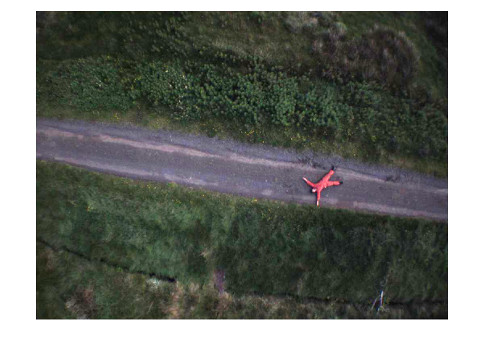
\includegraphics[width=0.48\textwidth]{fig/classimg.jpg} 
\label{fig:aerialimg}}
\subfigure[HOG classifier scores]{
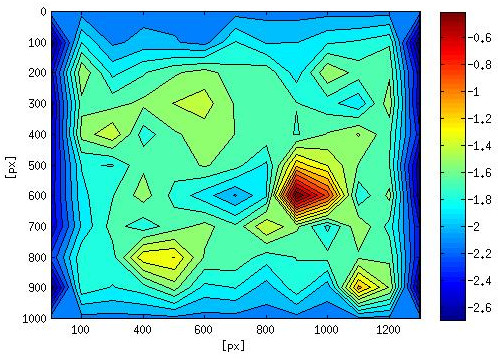
\includegraphics[width=0.48\textwidth]{fig/classscores.jpg}
\label{fig:classscores}}
\caption{Person detection from aerial images.\label{fig:persdetect}}
\end{figure}

The classifier model needs to be queried multiple times for each of the simulated image observation, so limiting its computational complexity is crucial to a successful integration into our simulations.
The UAV flying altitude has a direct effect on the size that a person in the field of view has on the camera image, therefore is the primary variable that affects the classifier ability to perform detections.
For these two reasons at present we focus on modelling the dependency between the flying altitude and the score returned by the classifier. In specific we model the scores as belonging to a Gaussian distribution for which with mean and standard deviation are simple functions of height.

If we plot the scores obtained by applying the HOG classifier to our dataset against altitude and we distinguish between positive (i.e. the person was in the window considered by the classifier) and negative examples (i.e. the was no person in the window), we obtain the graph of figure \ref{fig:datascores}.

At low altitudes ($<5m$) positive and negative example generate similar scores; at such altitudes only a part of the person is typically visible in the frame and this is not sufficient to elicit a strong classifier response since the HOG template we use is based on a whole body view of a person. As the altitude increases, positive examples are characterized by higher scores than negative ones as one would expect. At altitudes above $40m$ again the size of the person comes into play and simply the resolution is not sufficient to distinguish the person reliably from the background.

Is interesting to note also how the variation in scores decreases with altitude for the positive examples while it is almost independent from altitude for the negative examples. The latter can at least in part be explained by the multi-scale nature of the image features commonly present in a natural environment.   

\begin{figure}[ht]
\centering
\subfigure[Classifier scores as function of height, bars indicate $1\sigma$.]{
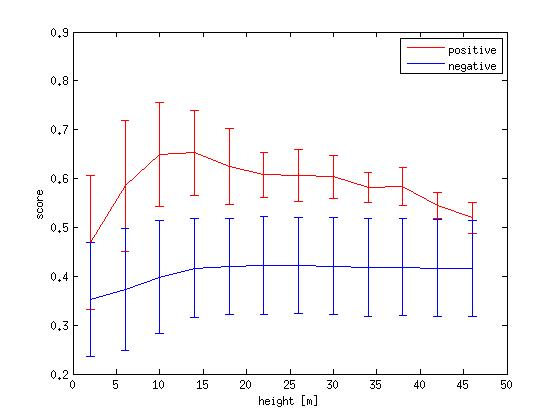
\includegraphics[width=0.46\textwidth]{fig/scoresbarplot.jpg}
\label{fig:datascores}}
\quad
\subfigure[Mean and standard deviation score as function of height, experimental vs. model.]{
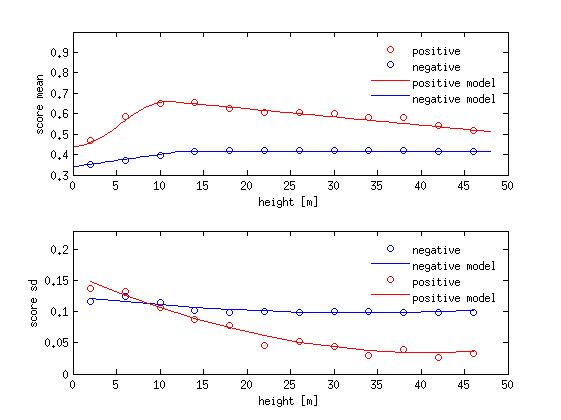
\includegraphics[width=0.46\textwidth]{fig/scoresmeansd.jpg}
\label{fig:scoresmodel}}
\caption{Scores as function of height.\label{fig:dataandmodels}}
\end{figure}

The relationship between scores and altitude  can be easily captured and simple analytic models can be devised for both the mean and the standard deviation of positive ($+$) and negative~($-$) scores:
\begin{eqnarray}
m^{+}_s &=& 
\left\{ 
\begin{array}{l l}
C^{+}_{m 0} + C^{+}_{m 1} \cos (\pi (1 + C^{+}_{m 2} h))  & \quad h<h_c \\
C^{+}_{m 3} +  C^{+}_{m 4} (h - h_c) + C^{+}_{m 5} & \quad h \geq h_c \label{eqn:meanpos}
\end{array}
\right.
\\
\sigma^{+}_s &=& C^{+}_{\sigma 0} + C^{+}_{\sigma 1} h+ C^{+}_{\sigma 2} h^2
\\ \nonumber
\\ 
m^{-}_s &=&
\left\{ 
\begin{array}{l l}
C^{-}_{m 0} + C^{-}_{m 1} h & \quad h<h_c \\
C^{-}_{m} & \quad h \geq h_c
\end{array}
\right.
\\
\sigma^{-}_s &=& C^{-}_{\sigma 0} + C^{-}_{\sigma 1} h+ C^{-}_{\sigma 2} h^2 \label{eqn:sigmaneg}
\end{eqnarray}
where $h$ is the UAV altitude and $C^{+}_{m 0},...,C^{+}_{m 5},C^{+}_{\sigma 0},...,C^{+}_{\sigma 2},C^{-}_{m 0},C^{-}_{m 1},C^{-}_{\sigma 0},...,C^{-}_{\sigma 2}$ are obtained by data fitting.

Within the simulator the UAV pose and the target locations are known, so it is possible to compute in which windows of the image frame the target will appear. Since the UAV height is known, to generate an observed score for a window we sample from a Gaussian distribution with mean and variance defined by equations \ref{eqn:meanpos}-\ref{eqn:sigmaneg}. We choose the parameters for positive scores if the target appears in the window, for negative scores otherwise.

Given the sampled score, the likelihood ratio for each window is easily obtained since the positive and negative models are Gaussians distributions with known means and standard deviations.
In practice for numerical reason we compute log likelihoods and therefore we return the difference between the positive and negative log likelihoods

\newpage

\section{Concentration Models}

This section gives more details about the dispersion models used for the plume modelling scenario; before starting it is useful to introduce some nomenclature:
\begin{longtable}{l l l}
$x,y,z$ & coordinates w.r.t. the global NED frame of reference & $m$\\
$x',y',z'$ & coordinates w.r.t. the wind frame of reference & $m$\\
$X_s,Y_s$ & coordinates of the source w.r.t. the global NED frame  & $m$\\
$x\prime_s,y'_s$ & coordinates of the source w.r.t. the wind frame of reference  & $m$\\
$Q_s$ & emission rate of source $s$ & $Kg/s$\\
$H_s$ & equivalent height of source $s$ & $m$\\
$u$ & constant magnitude of the wind speed & $m/s$\\
$S$ & number of sources & \\
$a$ & diffusion parameter & \\
$b$ & diffusion parameter & \\
$\alpha_w$ & wind direction (clockwise from north) & $rads$\\
$I_s$ & total number of puff for source $s$ & \\
$T^i_s$ & time at which puff $i$ of source $s$ was emitted & $s$\\
$Q^i_s$ & total amount of plume emitted by source $s$ at time $T^i$ & $Kg$\\
$\boldsymbol\Sigma$ & Gaussian concentration covariance matrix \\
\label{tab:naming2}
\end{longtable}

Several of the following models are more easily formulated in a frame of reference with origin in the global frame and aligned with the wind direction (wind frame). We denote such coordinate with $'$ and the transformation between global and wind frame is simply:
\begin{eqnarray}
x' &=& x \cos(\alpha_w) \\
y' &=& y \sin(\alpha_w).
\end{eqnarray}

\subsection{Gaussian Concentration Model} \label{3dgauss}

As a starting point for the plume modelling scenario discussed in section \ref{plumemodelling} it is very useful to define a concentration model that has a small number of parameter and that is straightforward to estimate. 
To this aim we chose a simple and familiar three dimensional Gaussian model for the concentration $c$ at a generic location $x,y,z$:
\begin{equation}\label{eqn:singlesourcegaussian}
c(x,y,z) = %\frac{1}{(2\pi)^{3/2}|\boldsymbol\Sigma|^{1/2}}
\exp\left(-\frac{1}{2}
\left[\begin{array}{c}
x-X_s\\
y-Y_s\\
z-H_s
\end{array} \right]^T{\boldsymbol\Sigma}^{-1}
\left[\begin{array}{c}
x-X_s\\
y-Y_s\\
z-H_s
\end{array} \right]
\right)
\end{equation}
where $\boldsymbol\Sigma$ is the usual covariance matrix which define the ellipsoid dimensions and principal axes and $X_s,Y_s,H_s$ is the source location.

In practical terms such concentration pattern would be produced by a source emitting at a constant rate in an environment were wind is not present; in such situation wind advection can be neglected and only the diffusive contribution from turbulent eddy motion in the atmosphere is considered. When specifying a covariance matrix which has eigenvectors of different magnitude we implicitly define that the diffusivity in the 3D space is non isotropic.

\subsection{Gaussian Dispersion Models}

In a more realistic situation than the one described in section \ref{3dgauss} wind should be considered since it generally has a strong influence on the plume dispersion.  

Under the following assumptions:
\begin{itemize}
\item constant wind (with magnitude $u$);
\item source with constant emission rate $Q$;
\item sufficiently long time scale of interest;
\item isotropic diffusion;
\item negligible ground penetration; 
\item negligible variations in topography;
\end{itemize}
the advection-diffusion flux equation that distinguish how the plume disperse in the environment has a closed form solution and the plume concentration can be easily computed (see \cite{stockie2011}).
The resulting concentration has a cone-like shape starting at the plume source and expanding downwind. Profile concentrations are symmetric about the plume centerline and have the shape of a Gaussian (see figure \ref{fig:winddisp}).
\begin{figure}[b!]
\centering
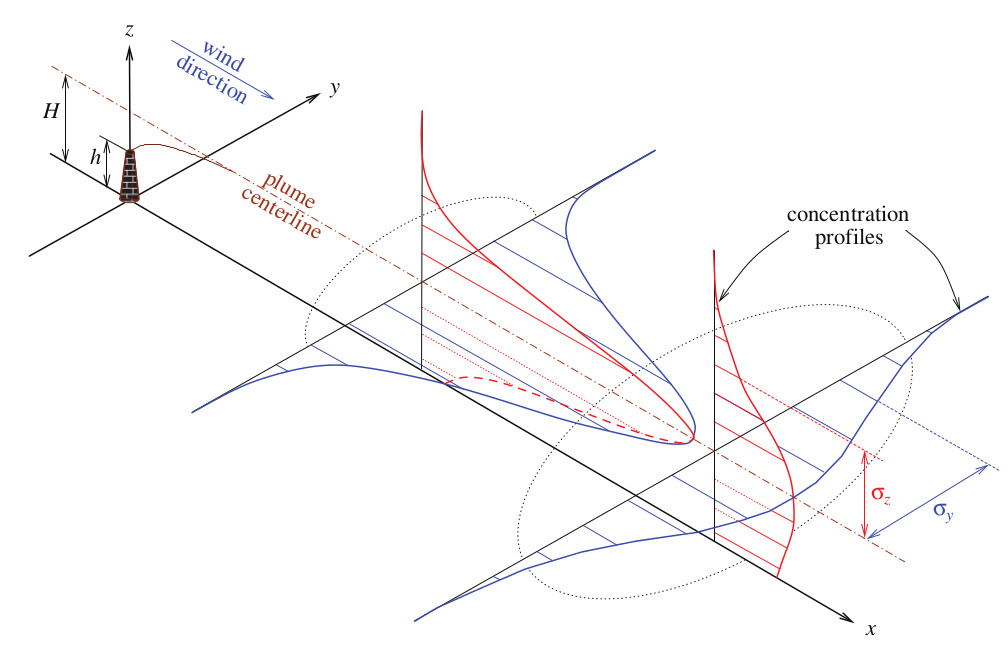
\includegraphics[width=0.8\textwidth]{fig/plumedistr.jpg}
\caption{Gaussian plume dispersion driven by wind (from\cite{stockie2011}).\label{fig:winddisp}}
\end{figure}

Analytically such a concentration is more easily written in the wind frame of reference (note the use of $x'$ and $y'$) as:
\begin{align}\label{eqn:singlesourcegaussiandispersion}
c(x',y',z) = &\frac{Q}{2\pi u a (x'-X'_s)^b}  \exp \left(-\frac{(y'-Y'_s)^2}{2 a (x'-X'_s)^b}\right) \nonumber \\
  & \left[ \exp \left(-\frac{(z-H_s)^2}{2 a (x'-X'_s)^b}\right) + \exp \left(-\frac{(z+H_s)^2}{2 a (x'-X'_s)^b}\right)\right]. 
\end{align}
where $a$ and $b$ are diffusion coefficients that regulate how the center line concentration evolves as the distance from the source increases.

\subsubsection{Multiple Sources Gaussian Dispersion Model}

In the case of a $S$ number of sources the total concentration can be computed by superposition of the effects of each of the single source:
\begin{align}\label{eqn:multiplesourcesgaussiandispersion}
c(x',y',z) = \sum_{s=1}^S c(x',y',z;X'_s,Y'_s,H_s,Q_s).
\end{align}
where $c(x',y',z;X'_s,Y'_s,H_s,Q_s)$ is nothing more equation \ref{eqn:singlesourcegaussiandispersion} in which $X'_s,Y'_s,H_s$ is the location of source $s$ and $Q_s$ is its emission rate.
We assume that the wind acting on each source is the same and therefore the wind frame of reference is unique.

\subsubsection{Single Source Gaussian Puff Dispersion Model}

The Gaussian dispersion model we just presented looks at the plume distribution over long time scales and assumes a constant emission rate from the source. 

It is fairly common however the case in which the source emits plume intermittently, the blob-like plume puffs are blown by the wind creating a time varying plume concentration.
A simple way of modelling this puff like dispersion is to assume that each puff $i$ generated by source $s$ has an emission time $T^i_s$ following which it moves downwind at the wind speed $u$. At a location $x',y',z$ and time $t$ the full concentration model is simply the superposition of all the puffs generated so far:
\begin{align}\label{eqn:singlesourcesgaussianpuffdispersion}
c(x',y',z,t) = & \sum_{i=1}^I \left\{ \frac{Q^i_s}{8(\pi a (x'-X'_s)^b)^{3/2}} \right. \nonumber \\
& \exp\left(-\frac{(x'-X'_s-u(t-T^i_s))^2+(y'-Y'_s)^2}{2 a (x'-X'_s)^b}\right) \nonumber \\
& \left. \left[\exp\left(-\frac{(z-H_s)^2}{2 a (x'-X'_s)^b}\right) + \exp\left(-\frac{(z+H_s)^2}{2 a (x'-X'_s)^b}\right)\right]\right\}
\end{align}
where $a$ and $b$ are the dispersion coefficients that we already encountered in equation \ref{eqn:singlesourcegaussiandispersion} and $Q^i_s$ is the amount of plume emitted with puff $i$ by source $s$. We sample $Q^i_s$ from a uniform distribution:
\begin{align}\label{eqn:qi}
Q^i_s \sim \mathcal{U}(q_m,q_M).
\end{align}


To fully define the model, the emission times need to be specified; in our settings we sample the inter-emission time $\tau^i$ from a exponential distribution with rate $\lambda$:
\begin{align}\label{eqn:ti}
T^i_s = T^{(i-1)}_s + \tau^i   \qquad \qquad \tau^i \sim Exp (\lambda), \quad T^0_s = 0.
\end{align}

\subsubsection{Multiple Sources Gaussian Puff Dispersion Model}

Even in the case of a time varying dispersion model, multiple sources can be considered. The total concentration can be computed by superposition:
\begin{align}\label{eqn:multiplesourcesgaussianpuffdispersion}
c(x',y',z,t) = \sum_{s=1}^S c(x',y',z,t;X'_s,Y'_s,H_s).
\end{align}
where $c(x',y',z,t;X'_s,Y'_s,H_s)$ is equation \ref{eqn:singlesourcesgaussianpuffdispersion} in which $X'_s,Y'_s,H_s$ is the location of source $s$ and $Q^i_s$ and $T^i_s$ are respectively sampled from an exponential and uniform distribution (i.e. equations \ref{eqn:qi}-\ref{eqn:ti}).
Again we implicitly assume that the wind acting on each source is the same and therefore the wind frame of reference is unique.


\begin{thebibliography}{1}

\bibitem{stockie2011} John M. Stockie {\em The Mathematics of
Atmospheric Dispersion Modeling}, {SIAM} Review, vol 53, no. 2, pages 349-372, May 2011.

\bibitem{dalal2005} N. Dalal, B. Triggs. {\em Histograms of Oriented Gradients for Human Detection}, Proceedings of the {IEEE} Conference on Computer Vision \& Pattern Recognition (CVPR), vol. II, pages 886-893, June 2005.

\bibitem{handa2012} Ankur Handa, Richard A. Newcombe, Adrien Angeli, Andrew J. Davison. {\em Real-Time Camera Tracking: When is High Frame-Rate Best?}, Proceedings of the European Conference on Computer Vision (ECCV), 2012.

\end{thebibliography}
  
\end{document}


